%! TEX program = xelatex
% 
% Template Proposal Tugas Akhir
% Program Studi Sistem dan Teknologi Informasi
% Sekolah Teknik Elektro dan Informatika
% Institut Teknologi Bandung
% 
% Dibuat oleh: IGB Baskara Nugraha 
% Email: baskara@itb.ac.id 
% 
% Last updated: 20 Oktober 2025
%
% Petunjuk penggunaan:
% 1. Ada 2 file utama, yaitu ProposalTA.tex (file ini) dan daftar-pustaka.bib (file daftar pustaka).
% 2. Sunting ProposalTA.tex sesuai dengan kebutuhan Anda.
% 3. Sunting atau generate isi daftar-pustaka.bib dengan referensi yang Anda gunakan, sesuai dengan format BibLaTeX.
% 4. Simpan kedua file tersebut dalam satu folder yang sama.
% 5. Kompilasi file ProposalTA.tex menggunakan XeLaTeX dan Biber (lihat urutan cara kompilasi di bawah).
% 6. Hasil kompilasi adalah file ProposalTA.pdf yang siap dicetak.
% 
% Urutan cara kompilasi (melalui command line):
% 1. xelatex ProposalTA.tex
% 2. biber ProposalTA      
% 3. xelatex  ProposalTA.tex
% 4. xelatex  ProposalTA.tex
%
% Catatan:
% - Pastikan Anda telah menginstal paket-paket LaTeX yang diperlukan, termasuk
%   biblatex-chicago dan fontspec.
% - Gunakan editor LaTeX yang mendukung XeLaTeX, seperti TeXstudio, Overleaf, atau lainnya.
% - Jika meenggunakan Visual Studio Code sebagai editor, pastikan mengatur "latex-workshop.latex.tools" dan
%   "latex-workshop.latex.recipes" untuk mendukung XeLaTeX dan Biber dengan cara menambahkan konfigurasi berikut:
%   "latex-workshop.latex.tools": [ 
%       {
%           "name": "xelatex",
%           "command": "xelatex",
%           "args": [
%               "-synctex=1",
%               "-interaction=nonstopmode",
%               "-file-line-error",
%               "%DOC%"
%           ]
%       },
%       {
%           "name": "biber",
%           "command": "biber",
%           "args": [
%               "%DOCFILE%"
%           ]
%       }
%   ],
%   "latex-workshop.latex.recipes": [
%       {
%           "name": "xelatex -> biber -> xelatex*2",
%           "tools": [
%               "xelatex",
%               "biber",
%               "xelatex",
%               "xelatex"
%           ]
%       }
%   ]
% - Untuk referensi lebih lanjut tentang penggunaan BibLaTeX dengan gaya Chicago, silakan merujuk ke dokumentasi resmi BibLaTeX.
%   https://ctan.org/pkg/biblatex-chicago
% - Untuk referensi lebih lanjut tentang penggunaan XeLaTeX dan fontspec, silakan merujuk ke dokumentasi resmi fontspec.
%   https://ctan.org/pkg/fontspec
% - Selamat menyusun proposal tugas akhir Anda!
%
\documentclass[12pt,a4paper,oneside]{book}

% ==========================================
% BASIC PACKAGES
% ==========================================
\usepackage[utf8]{inputenc} % for UTF-8 encoding
\usepackage{fontspec} % for font selection
\setmainfont{Times New Roman} % set main font to Times New Roman
\usepackage[a4paper, left=4cm, right=3cm, top=3cm, bottom=3cm]{geometry} % set page margins
\usepackage[indonesian]{babel} % untuk bahasa Indonesia
\usepackage{csquotes} % for context-sensitive quotation facilities
\usepackage{setspace} % for line spacing
\onehalfspacing % spasi 1.5
\usepackage{graphicx} % for images
\usepackage{caption} % for customizing captions
\usepackage{subcaption} % for sub-figures
\usepackage{hyperref} % for hyperlinks
\usepackage{titlesec} % for customizing titles
\usepackage{tocloft} % for customizing table of contents
\usepackage{lipsum} % for dummy text (lorem ipsum text)
\usepackage{floatrow} % for customizing float (figure and table) positions
\usepackage{listings} % for code listing
\usepackage{amsmath} % for math
\usepackage{amssymb} % for math symbols
\usepackage[shortlabels]{enumitem} % for customizing lists
\setlist[enumerate]{nosep, topsep=-10pt} % mengurangi spasi antar item dan atas bawah daftar
\setlist[itemize]{nosep, topsep=-10pt} % mengurangi spasi antar item dan atas bawah daftar
\usepackage[skip=12pt]{parskip}
\usepackage{longtable}
\usepackage{booktabs}
\usepackage[id-ID]{datetime2}


\setcounter{tocdepth}{4} % kedalaman daftar isi sampai subsubbab
\setcounter{secnumdepth}{4} % kedalaman penomoran sampai subsubbab


% ==========================================
% SITASI DAN DAFTAR PUSTAKA (MENGGUNAKAN CHICAGO MANUAL OF STYLE)
% ==========================================
\usepackage[
    backend=biber,
    authordate,
    language=english,
    autolang=other
]{biblatex-chicago}

\addbibresource{daftar-pustaka.bib}

% ==========================================
% Ubah istilah bahasa Inggris di daftar pustaka ke Bahasa Indonesia
% ==========================================
\DefineBibliographyStrings{english}{
  and          = {dan},
  andothers    = {dkk.},
  editor       = {penyunting},
  editors      = {penyunting},
  translator   = {penerjemah},
  byeditor     = {disunting oleh},
  bytranslator = {diterjemahkan oleh},
  in           = {dalam},
  edition      = {edisi},
  pages        = {hal.},
  page         = {hal.},
  volume       = {vol.},
  number       = {no.},
  urlseen      = {diakses pada},
  url          = {tautan},
}

% ==========================================
% Pastikan \cite() menampilkan (Penulis Tahun)
% ==========================================
\let\oldcite\cite
\renewcommand{\cite}{\parencite}

% ==========================================
% Atur pemisah nama penulis agar lebih natural dalam Bahasa Indonesia
% ==========================================
\renewcommand*{\finalandcomma}{} % hilangkan koma sebelum 'dan'


% ==========================================
% TAMPILAN
% ==========================================
\hypersetup{
    colorlinks=true,
    linkcolor=black,
    citecolor=black,
    urlcolor=black
}

% -- No Header dan No Footer ---
\pagestyle{plain}

% --- Ubah nama daftar listing ke "DAFTAR ALGORITMA" ---
% --- Harus diletakkan sebelum \begin{document} ---
\renewcommand{\lstlistlistingname}{\centering\normalsize DAFTAR KODE} 
\renewcommand{\lstlistingname}{Kode}
\lstset{basicstyle=\ttfamily\footnotesize,breaklines=true}
%\captionsetup[lstlisting]{justification=raggedright,singlelinecheck=false}


\renewcommand \cftchapdotsep{4.5}

% ==========================================
% AWAL DOKUMEN
% ==========================================
\begin{document}

% ==========================================
% HALAMAN JUDUL
% ==========================================
\begin{titlepage}
\begin{center}

    
    \vspace*{2cm}
    
    {\Large\bfseries PERANCANGAN SISTEM INFORMASI AKADEMIK BERBASIS WEB}\\
     \vspace{4cm}

    {\Large \textbf{Proposal Tugas Akhir}}\\


    \vspace{2cm}
    
    
    {\large Oleh}\\[0.3cm]
    \textbf{
    {\large John Doe}\\
    {\large 18299000}
    }\\

    \vspace{2cm}
    
    \begin{figure}[h]
    \centering
    
\includegraphics[width=0.2\textwidth]{image/ganesha.jpg}
    \end{figure}
    
    
    % \vspace{1cm}
    \vfill

    \textbf{
    {\large PROGRAM STUDI SISTEM DAN TEKNOLOGI INFORMASI}\\
    {\large SEKOLAH TEKNIK ELEKTRO DAN INFORMATIKA}\\
    {\large INSTITUT TEKNOLOGI BANDUNG}\\
    {\large \DTMlangsetup{showdayofmonth=false,showmonthname=true,showyear=true}\today}
    }
\end{center}
\end{titlepage}



% ==========================================
% LEMBAR PENGESAHAN 
% ==========================================
\newpage
\thispagestyle{empty}
\pagenumbering{gobble}
\begin{center}
  \textbf{\large LEMBAR PENGESAHAN}\\[1cm]
  \vspace*{1.5cm}
    
  {\large\bfseries PERANCANGAN SISTEM INFORMASI AKADEMIK BERBASIS WEB}\\
     \vspace{2cm}

  {\Large \textbf{Proposal Tugas Akhir}}\\


  \vspace{1.5cm}
    
    
  {\large Oleh}\\[0.3cm]
    \textbf{
    {\large John Doe}\\
    {\large 18299000}
  }\\
    
  \vspace{0.5cm}
 
  {\large Program Studi Sistem dan Teknologi Informasi}\\
  {\large Sekolah Teknik Elektro dan Informatika}\\
  {\large Institut Teknologi Bandung}\\

  \vspace{1.5cm}

  Proposal Tugas Akhir ini telah disetujui dan disahkan\\ 
  di Bandung, pada tanggal \today\\[1cm]

% ==========================================
% Versi 1 pembimbing (default)
% ==========================================
	Pembimbing  \\[3cm]
	Dr. Ir. John Doe, M.T.   \\[0.2cm]
	NIP. 123456789 
% ==========================================

\end{center}

\vspace{1cm}
\noindent

% ==========================================
% Jika ada 2 pembimbing TA, uncomment dan edit 
% tabular di bawah ini. Kemudian, comment out atau hapus
% bagian versi 1 pembimbing di atas.
% ==========================================

%\begin{tabular}{p{1cm}p{7cm}p{7cm}}
%   & Pembimbing 1 & Pembimbing 2 \\[3cm]
%   & Dr. Ir. John Doe, M.T. & Dr. Mary Doe, M.Sc. \\[0.2cm]
%   &  NIP. 123456789 & NIP. 987654321
%\end{tabular}



% -- Change page number style to roman ---
\pagenumbering{roman} 


% ==========================================
% DAFTAR ISI, TABEL, GAMBAR
% ==========================================
% --- DAFTAR ISI ---
\makeatletter
\renewcommand{\tableofcontents}{%
  \clearpage
  \thispagestyle{plain}% no header
  \begin{center}
    {\large\bfseries\MakeUppercase{\contentsname}\par}
  \end{center}
  \vskip 1em
  \@starttoc{toc}%
}
\makeatother

\newpage
\renewcommand{\cfttoctitlefont}{\hfill\large\bfseries\MakeUppercase}
\renewcommand{\cftaftertoctitle}{\hfill}
\tableofcontents
%\addcontentsline{toc}{chapter}{DAFTAR ISI}

% --- DAFTAR GAMBAR ---
\newpage
\renewcommand{\cftloftitlefont}{\hfill\large\bfseries\MakeUppercase}
\renewcommand{\cftafterloftitle}{\hfill}
\listoffigures
\addcontentsline{toc}{chapter}{DAFTAR GAMBAR}

% --- DAFTAR TABEL ---
\newpage
\renewcommand{\cftlottitlefont}{\hfill\large\bfseries\MakeUppercase}
\renewcommand{\cftafterlottitle}{\hfill}
\listoftables
\addcontentsline{toc}{chapter}{DAFTAR TABEL}

% --- DAFTAR LISTING (ALGORITMA, PSEUDOCODE, SOURCE CODE) ---
\newpage

\lstlistoflistings
\addcontentsline{toc}{chapter}{\lstlistlistingname}

\mainmatter
% --- FORMAT TAMPILAN JUDUL BAB, SUBBAB, JUDUL GAMBAR DAN TABEL ---
% --- Judul Bab ---
\titleformat{\chapter}[display]
      {\centering\normalfont\large\bfseries} % Commands for the entire chapter title
      {\MakeUppercase \chaptertitlename\ \thechapter}{0pt}{\large} % Chapter number format
\renewcommand\thechapter{\Roman{chapter}}
% --- Judul Subbab dan Subsubbab ---
\titleformat{\section}
	{\normalfont\bfseries}
	{\thesection}{1em}{}
\titleformat{\subsection}
	{\normalfont\bfseries}
	{\thesubsection}{1em}{}
\titleformat{\subsubsection}
	{\normalfont\bfseries}
	{\thesubsubsection}{1em}{}


% --- Format judul gambar dan tabel ---
\captionsetup[figure]{labelsep=space}
\captionsetup[table]{labelsep=space}
\floatsetup[table]{capposition=top}
\captionsetup[lstlisting]{labelsep=space}
\floatsetup[lstlisting]{capposition=top}

% --- Atur indentasi paragraf ---
\setlength{\parindent}{0pt}
% -- Change page number style to arabic ---
\pagenumbering{arabic} 

% ==========================================
% BAB I PENDAHULUAN
% ==========================================
\chapter{PENDAHULUAN}
\label{chap:pendahuluan}
% --- Latar Belakang ---
\section{Latar Belakang}
Latar Belakang menjelaskan dasar pemikiran, motivasi, kebutuhan, alasan, atau urgensi pemilihan masalah tugas akhir. Subbab ini berisi penjelasan ringkas tentang kondisi atau situasi yang ada saat ini terkait dengan topik yang dibahas. Tujuan utamanya adalah untuk memberikan informasi secukupnya kepada pembaca agar memahami topik yang akan dibahas. Dalam subbab ini, jelaskan hal-hal berikut ini:
\begin{enumerate}
\item	Kondisi atau situasi topik yang dibahas beserta permasalahannya, misalnya tentang pengelolaan informasi di puskesmas daerah pedesaan dan masalah yang dihadapi.
\item	Berbagai solusi yang telah diterapkan atau solusi yang tersedia dan memungkinkan untuk diterapkan untuk menyelesaikan masalah tersebut.
\end{enumerate}

% --- Rumusan Masalah ---
\section{Rumusan Masalah}
Rumusan Masalah berisi masalah utama yang dibahas dalam tugas akhir. Rumusan masalah yang baik memiliki struktur sebagai berikut:
\begin{enumerate}
\item	Pokok persoalan dari kondisi atau situasi yang ada saat ini. Dengan kata lain, jelaskan kelemahan atau kekurangan dari kondisi, situasi, atau solusi yang dijelaskan pada latar belakang. Ini merupakan pokok rumusan masalah.
\item	Elaborasi lebih lanjut urgensi penyelesaian masalah tersebut (mengapa penting untuk diselesaikan dan akibat yang dapat terjadi jika tidak diselesaikan).
\item	Usulan singkat terkait dengan solusi yang ditawarkan untuk menyelesaikan persoalan.
Penting untuk diperhatikan bahwa persoalan yang dideskripsikan pada subbab ini akan dipertanggungjawabkan di bab Evaluasi (apakah terselesaikan atau tidak).
\end{enumerate}

% --- Tujuan ---
\section{Tujuan}
Tuliskan tujuan utama dan/atau tujuan detail yang akan dicapai dalam pelaksanaan tugas akhir. Fokuskan pada hasil akhir yang ingin diperoleh setelah tugas akhir diselesaikan, terkait dengan penyelesaian persoalan pada rumusan masalah. Penting untuk diperhatikan bahwa tujuan yang dideskripsikan pada subbab ini akan dipertanggungjawabkan di akhir pelaksanaan tugas akhir apakah tercapai atau tidak. Tuliskan kriteria keberhasilan tugas akhir ini.

% --- Batasan Masalah ---
\section{Batasan Masalah}
Tuliskan batasan-batasan yang diambil dalam pelaksanaan tugas akhir. Batasan ini dapat dihindari (bersifat opsional, tidak perlu ada) jika topik atau judul tugas akhir dibuat cukup spesifik.

% --- Metodologi Pengerjaan TA ---
\section{Metodologi}
Tuliskan semua tahapan yang akan dilalui selama pelaksanaan tugas akhir. Tahapan ini spesifik untuk menyelesaikan persoalan tugas akhir. Khusus untuk penyusunan proposal ini, jelaskan secara detail:
\begin{enumerate}
\item	Tahapan investigasi pengumpulan fakta di latar belakang untuk merumuskan masalah.
\item	Langkah-langkah pencarian, pengelompokan, dan penapisan literatur atau sumber informasi untuk mengumpulkan informasi yang relevan tentang topik yang diangkat, termasuk teori (konsep atau teori apa saja yang perlu dicari), hal-hal yang telah dicapai oleh orang lain (cara mencari dan kata kuncinya), dan berbagai informasi pendukung, untuk mencari solusi terhadap masalah yang dibahas. Gunakan metodologi yang tepat dalam menggali informasi dan dokumentasikan prosesnya (termasuk rekaman wawancara atau survei) di dalam Lampiran, termasuk tautan ke video atau foto. Hasil penggalian informasi ini akan dijelaskan secara sistematis di Bab II Studi Literatur.
\end{enumerate}
% ==========================================
% BAB II STUDI LITERATUR
% ==========================================
\chapter{STUDI LITERATUR}
\label{chap:studi-literatur}
\section{Penulisan Gambar, Tabel, Rumus, dan Kode}
\lipsum[1]

\subsection{Gambar}
Contoh gambar dapat dilihat pada Gambar \ref{gambar:jaringan}. Gambar dan judulnya diposisikan di tengah. Nomor gambar tidak diakhiri tanda titik. Gambar tersebut dibuat menggunakan aplikasi draw.io dan disimpan ke format PNG setelah dengan zoom setting pada angka 300\%. Ukuran gambar yang ditampilkan dapat diatur dengan mengubah nilai \textit{width} dalam sintaks \textit{includegraphics}.

\begin{figure}[t] % pilihan opsi yang disarankan: t = top, b = bottom, h = here
	\centering
  \captionsetup{justification=centering}
    	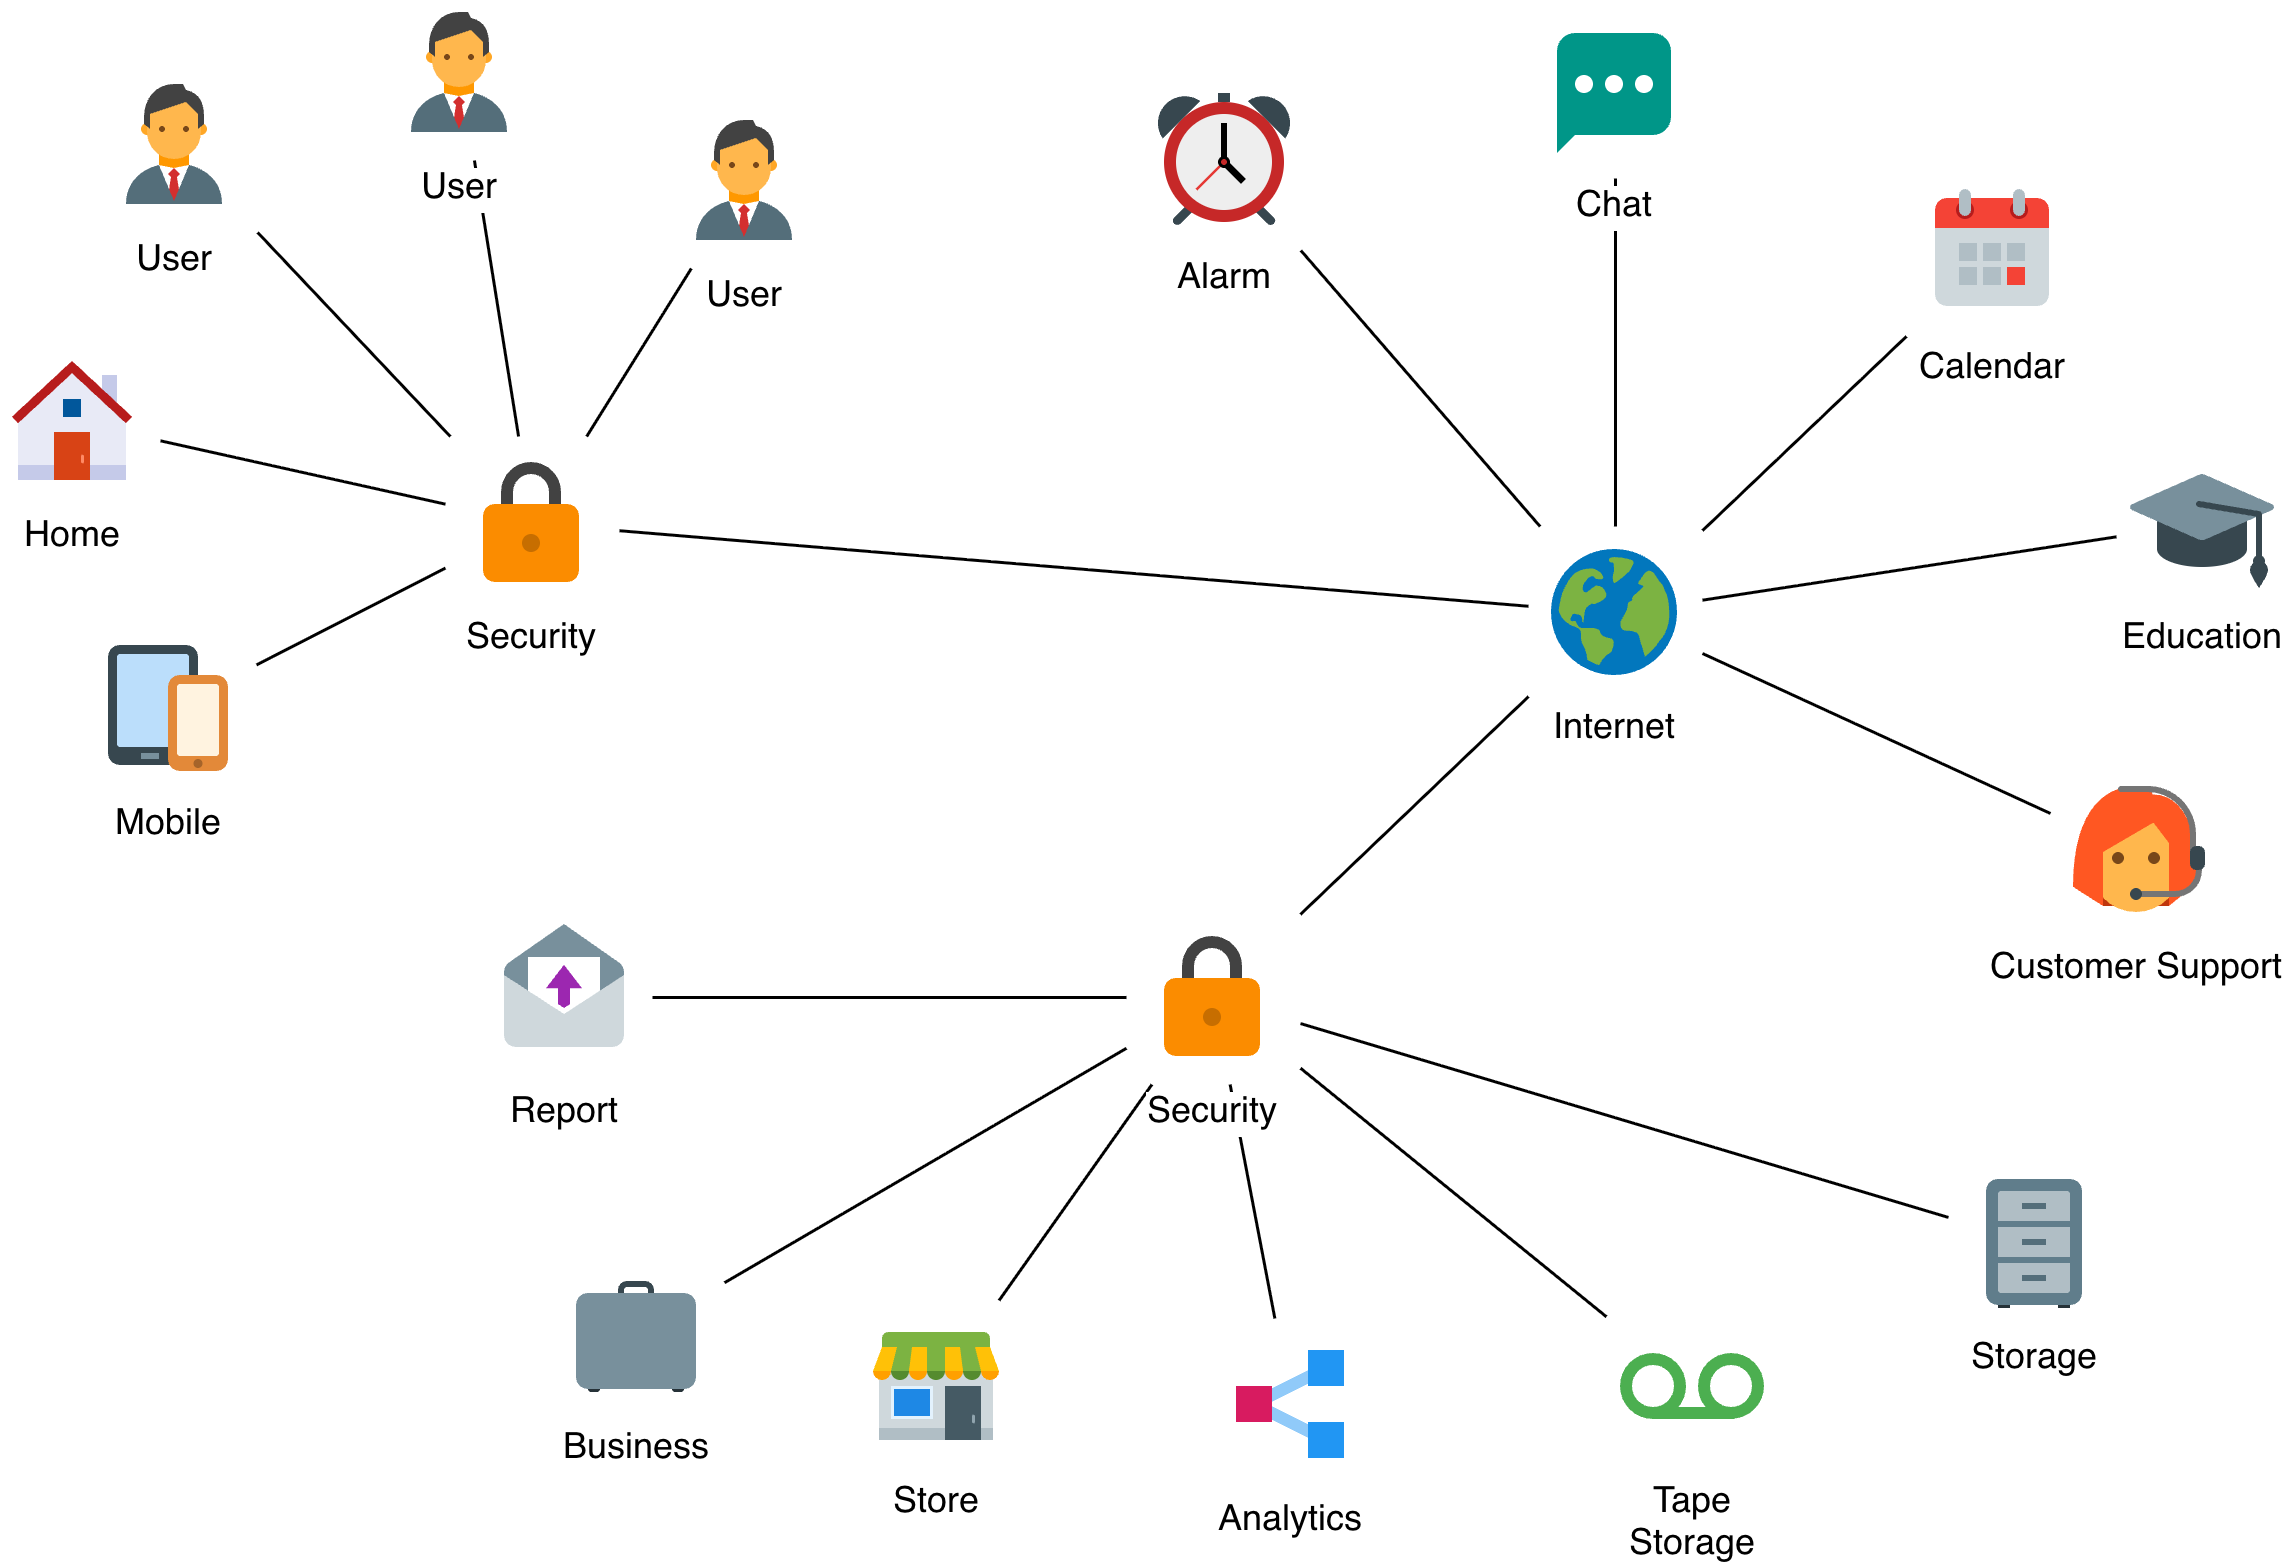
\includegraphics[width=0.7\textwidth]{gambar1.png}
	\caption{Contoh gambar jaringan}
	\label{gambar:jaringan}
\end{figure}

Gambar umumnya tidak jelas atau kabur jika gambar tersebut:
\begin{enumerate}[a.]
  \item diperoleh dari hasil cropping pada suatu halaman buku atau situs web;
  \item hasil pembesaran gambar yang gambar aslinya sebenarnya berukuran kecil; atau
  \item disimpan dalam resolusi kecil
\end{enumerate}
Ketidakjelasan gambar ini dapat dilihat pada garis-garis diagram yang tidak tegas dan tulisan-tulisan dalam gambar yang tampak kabur dan kurang jelas terbaca.

Untuk mendapatkan gambar yang tidak kabur (\textit{blur}), langkah-langkah berikut dapat digunakan:
\begin{enumerate}[(a)]
\item Gambar yang didapat di suatu pustaka atau referensi sebaiknya digambar ulang, misalnya menggunakan PowerPoint, Canva, Figma, draw.io, atau yang lainnya.
\item Jika diagram atau ilustrasi digambar menggunakan draw.io, saat gambar disimpan ke format PNG atau JPG (\textit{export as}), lakukan \textit{zoom} ke minimal 300\% (\textit{the default value is} 100\%). 
\item Jika diagram digambar dengan menggunakan PowerPoint, gambar dapat langsung di-\textit{copy-paste} ke Word.
\end{enumerate}

\subsection{Tabel}
Tabel ada dua jenis, yaitu tabel yang bisa termuat dalam satu halaman dan tabel yang sangat panjang sehingga tidak muat dalam satu halaman.
\subsubsection{Tabel yang Muat dalam Satu Halaman}
Contoh tabel dapat dilihat pada Tabel \ref{tbl:harga1} dan \ref{tbl:harga2}. Tabel dan judulnya dibuat rata kiri dan judul tabel diletakkan di atas tabel. Usahakan tabel dapat ditulis dalam satu halaman, tidak terpotong ke halaman berikutnya.

\begin{table}[t] % pilihan opsi yang disarankan: t = top, b = bottom, h = here
  \begin{tabular}{ | p{2cm} | p{2cm} | p{3cm} |}
	\hline
	Nama 	& Satuan 		& Harga \\
	\hline
	Buku 	& Exemplar	& 25000 \\
	Komputer	& Unit		& 2500000 \\
	Pensil	& Buah		& 118900 \\
	\hline
	\end{tabular}
\caption{Tabel harga bahan pokok}
\label{tbl:harga1}
\end{table}

\begin{table}[t] % pilihan opsi yang disarankan: t = top, b = bottom, h = here
	\begin{tabular}{ | l | c | r | }
	\hline
	Nama 	& Satuan 		& Harga \\
	\hline
	Buku 	& Exemplar	& 25000 \\
	Komputer	& Unit		& 2500000 \\
	Pensil	& Buah		& 118900 \\
	\hline
	\end{tabular}
\caption{Tabel harga bahan sekunder}
\label{tbl:harga2}
\end{table}

\subsubsection{Tabel yang Sangat Panjang}
Jika tabel terlalu panjang sehingga tidak muat dalam satu halaman, gunakan paket 
\textit{longtable} untuk membuat tabel yang dapat terpotong ke halaman berikutnya, 
seperti pada Tabel \ref{tbl:longtable1}.

\begin{longtable}{@{\extracolsep{\fill}} l c r r}
\caption{Comprehensive Data Table Example}\label{tbl:longtable1} \\
\toprule
\textbf{ID} & \textbf{Name} & \textbf{Score} & \textbf{Rank} \\
\midrule
\endfirsthead

\caption*{Comprehensive Data Table Example (lanjutan)} \\
\toprule
\textbf{ID} & \textbf{Name} & \textbf{Score} & \textbf{Rank} \\
\midrule
\endhead

\midrule
\multicolumn{4}{r}{\textit{Bersambung ke halaman berikutnya}} \\
\bottomrule
\endfoot

\bottomrule
\endlastfoot

% === Table Data ===
1 & Alice Smith & 89 & 5 \\
2 & Bob Johnson & 93 & 3 \\
3 & Carol Davis & 95 & 2 \\
4 & Daniel Wilson & 88 & 6 \\
5 & Eve Thompson & 97 & 1 \\
6 & Frank Brown & 85 & 7 \\
7 & Grace Lee & 91 & 4 \\
8 & Henry Miller & 80 & 9 \\
9 & Irene Garcia & 83 & 8 \\
10 & Jack Robinson & 78 & 10 \\
% Repeat with more rows to make it long
11 & Kevin Harris & 76 & 11 \\
12 & Laura Martin & 75 & 12 \\
13 & Michael Clark & 74 & 13 \\
14 & Natalie Lewis & 73 & 14 \\
15 & Olivia Walker & 72 & 15 \\
16 & Peter Hall & 71 & 16 \\
17 & Quinn Allen & 70 & 17 \\
18 & Rachel Young & 69 & 18 \\
19 & Samuel King & 68 & 19 \\
20 & Tina Wright & 67 & 20 \\
21 & Uma Scott & 66 & 21 \\
22 & Victor Green & 65 & 22 \\
23 & Wendy Adams & 64 & 23 \\
24 & Xavier Nelson & 63 & 24 \\
25 & Yolanda Carter & 62 & 25 \\
26 & Zachary Perez & 61 & 26 \\
27 & Amelia Baker & 60 & 27 \\
28 & Benjamin Rivera & 59 & 28 \\
29 & Charlotte Rogers & 58 & 29 \\
30 & David Murphy & 57 & 30 \\
31 & Ethan Cooper & 56 & 31 \\
32 & Fiona Reed & 55 & 32 \\
33 & George Bailey & 54 & 33 \\
34 & Hannah Cox & 53 & 34 \\
35 & Isaac Howard & 52 & 35 \\
36 & Julia Ward & 51 & 36 \\
37 & Kyle Flores & 50 & 37 \\
38 & Lily Bell & 49 & 38 \\
39 & Mason Sanders & 48 & 39 \\
40 & Nora Patterson & 47 & 40 \\
41 & Owen Ramirez & 46 & 41 \\
42 & Penelope Torres & 45 & 42 \\
43 & Quentin Foster & 44 & 43 \\
44 & Rebecca Gonzales & 43 & 44 \\
45 & Sebastian Bryant & 42 & 45 \\
46 & Taylor Alexander & 41 & 46 \\
47 & Ursula Russell & 40 & 47 \\
48 & Vincent Griffin & 39 & 48 \\
49 & William Diaz & 38 & 49 \\
50 & Zoe Simmons & 37 & 50 \\
% (You can easily extend this list to hundreds of rows)
\end{longtable}

\subsubsection{Rumus}
Contoh rumus matematika dapat ditulis seperti pada Persamaan \ref{eq:contoh1} di bawah ini. 
Penomoran persamaan diletakkan di sebelah kanan, dan rumus ditulis dalam mode \textit{display math}.
\begin{equation}
E = mc^2
\label{eq:contoh1}
\end{equation}

Contoh lain penulisan rumus matematika yang lebih kompleks dapat ditulis seperti pada Persamaan \ref{eq:rumus2}.

\begin{align}
f(x) &= ax^2 + bx + c \\
f'(x) &= \frac{d}{dx}(ax^2 + bx + c) \notag \\ % tidak menampilkan nomor pada baris ini
      &= 2ax + b \label{eq:rumus2}
\end{align}

Jika rumus terlalu panjang untuk ditulis dalam satu baris, gunakan lingkungan \textit{multline} seperti pada Persamaan \ref{eq:rumus3} di bawah ini.
\begin{multline} 
y = a_0 + a_1x + a_2x^2 + a_3x^3 + a_4x^4 + a_5x^5 + a_6x^6 + a_7x^7 \\
    + a_8x^8 + a_9x^9 + a_{10}x^{10} \label{eq:rumus3}
\end{multline}

Jika ada penurunan rumus yang terdiri dari beberapa baris, namun tidak memerlukan penomoran pada setiap baris, gunakan lingkungan \textit{align*}, misalnya:

\begin{align*} 
S &= \sum_{i=1}^{n} i^2 \\
  &= 1^2 + 2^2 + 3^2 + \cdots + n^2 \\
  &= \frac{n(n + 1)(2n + 1)}{6}
\intertext{Contoh lainnya adalah rumus untuk mencari nilai rata-rata fungsi $f(x)$ pada interval $[p, q]$:}
\bar{f} &= \frac{1}{q - p} \int_{p}^{q} f(x) \, dx \\
        &= \frac{1}{q - p} \int_{p}^{q} (ax^2 + bx + c) \, dx \\
        &= \frac{1}{q - p} \left[ \frac{a}{3}x^3 + \frac{b}{2}x^2 + cx \right]_p^q \\
        &= \frac{a(q^3 - p^3)}{3(q - p)} + \frac{b(q^2 - p^2)}{2(q - p)} + c \label{eq:rumus4}
\end{align*}



\subsection{Algoritma, Pseudocode, atau Kode}
Contoh penulisan algoritma atau pseudocode dapat ditulis seperti pada Kode \ref{alg:contoh1} di bawah ini. 
Gunakan paket \textit{listings} untuk menulis source code dalam bahasa pemrograman tertentu, seperti pada Kode \ref{lst:contoh1}. 


% -- Example of pseudocode and source code listing --
% -- Gunakan minipage agar listing tidak terpotong ke halaman berikutnya --
\begin{minipage}{\textwidth} 
\begin{lstlisting}[frame=lines, captionpos=t, caption={Contoh pseudocode}, label={alg:contoh1}]
ALGORITHM HelloWorld
   PRINT "Hello, World!"
END ALGORITHM
\end{lstlisting}
\end{minipage}

\begin{minipage}{\textwidth}
\begin{lstlisting}[language=Python, frame=single, caption={Contoh source code Python}, captionpos=t, label={lst:contoh1}]
def hello_world():
    print("Hello, World!")       
hello_world()
\end{lstlisting}
\end{minipage}


\section{Beberapa Kesalahan Penulisan yang Sering Terjadi}
\subsection{Penggunaan Kata "di mana" atau "dimana"}
Banyak yang menuliskan kata "di mana" atau "dimana" sebagai pengganti kata "which" dalam bahasa Inggris. 
Padahal, penggunaan kata "di mana" atau "dimana" tidak tepat dalam konteks tersebut. Demikian juga untuk kata serupa, misalnya "yang mana".
Kata "di mana" atau "dimana" ini harus diganti dengan kata lain, seperti "dengan", "tempat", "yang", dan sebagainya tergantung kalimatnya.
Penjelasan lengkap dapat dilihat pada \autocite{BPBI}.

\subsection{Penggunaan Kata "sedangkan" dan "sehingga"}

\begin{table}[t]
  \begin{tabular}{|c|l|l|}
  \hline
  Kata & Salah & Benar \\ \hline
  sedangkan & \begin{tabular}[c]{@{}c@{}}Sedangkan sistem lama masih\\ digunakan oleh banyak pengguna.\end{tabular} & \begin{tabular}[c]{@{}c@{}}Sistem lama masih digunakan\\ oleh banyak pengguna,\\ sedangkan sistem baru belum siap.\end{tabular} \\ \hline
  sehingga & \begin{tabular}[c]{@{}c@{}}Sehingga sistem lama masih\\ digunakan oleh banyak pengguna.\end{tabular} & \begin{tabular}[c]{@{}c@{}}Sistem lama masih digunakan\\ oleh banyak pengguna sehingga\\ sistem baru belum siap.\end{tabular} \\ \hline
  \end{tabular}
  \caption{Contoh penggunaan kata "sedangkan" dan "sehingga"}
  \label{tbl:sedangkan_sehingga}
\end{table}

Kata "sedangkan" dan "sehingga" adalah kata hubung atau konjungsi. 
Konjungsi adalah kata atau ungkapan yang menghubungkan satuan bahasa 
(kata, frasa, klausa, dan kalimat). 
Konjungsi dapat dibagi menjadi konjungsi intrakalimat dan antarkalimat.  
Kata "sedangkan" menghubungkan dua klausa yang bersifat kontrasif, 
sedangkan "sehingga" menghubungkan dua klausa yang bersifat kausal. 
Dalam ragam formal, kata hubung “sedangkan” dan “sehingga” hanya dapat digunakan 
sebagai konjungsi intrakalimat sehingga kedua konjungsi itu \textbf{tidak dapat diletakkan pada awal kalimat}.
Selain itu, penggunaan kata "sedangkan" harus didahului oleh koma (,), sedangkan kata "sehingga" tidak perlu didahului oleh koma (,).
Contoh penggunaan yang benar dan salah dapat dilihat pada Tabel \ref{tbl:sedangkan_sehingga}.


\subsection{Penggunaan Istilah yang Tidak Baku}
Ada beberapa istilah yang sering digunakan dalam pembicaraan sehari-hari, tetapi tidak baku dalam penulisan ilmiah.
Beberapa istilah tersebut antara lain:
\begin{enumerate}
  \item analisa $\rightarrow$ analisis
  \item eksisting atau existing $\rightarrow$ yang ada atau saat ini
  \item bisnis proses $\rightarrow$ proses bisnis
  \item user $\rightarrow$ pengguna
  \item system $\rightarrow$ sistem
  \item database $\rightarrow$ basis data
  \item aktifitas $\rightarrow$ aktivitas
  \item efektifitas $\rightarrow$ efektivitas
  \item sosial media $\rightarrow$ media sosial
\end{enumerate}

\subsection{Pemisah Desimal dan Ribuan}
Tanda pemisah desimal dalam bahasa Indonesia adalah tanda koma, contoh:
\begin{enumerate}
  \item (Salah) Akurasi naik menjadi 50.6\% 
  \item (Benar) Akurasi naik menjadi 50,6\% 
\end{enumerate}

\subsection{Daftar atau \textit{List}}
Ada beberapa aturan penulisan daftar atau \textit{list} yang perlu diperhatikan, antara lain:
\begin{enumerate}[a)]
\item Jika memungkinkan, hindari penggunaan “bullet points” atau sejenisnya. Sebaiknya, gunakan angka (1, 2, 3, ...) atau huruf (a, b, c, …). Dengan demikian, pembaca dapat dengan mudah melihat jumlah \textit{item} atau \textit{list}. 
\item Jika dalam daftar hanya ada satu item, tidak perlu menggunakan nomor urut.
\item Penjelasan atau deskripsi suatu item sebaiknya menyatu dengan judul item tersebut, tidak berbeda halaman. Contoh yang salah: judul item ada di halaman 10, namun deskripsinya di halaman 11. Sebaiknya pindahkan judul tersebut ke halaman 11.
\item Jika penjelasan atau deskripsi suatu item cukup panjang, misalnya lebih dari 1 halaman atau terdiri atas beberapa paragraf, sebaiknya setiap item tersebut dijadikan judul subbab, kecuali jika level subbab sudah mencapai level 4. 
\end{enumerate}

\subsection{Penggunaan Kata "masing-masing" dan "setiap"}
Kata “masing-masing” digunakan di belakang kata yang diterangkan, misalnya 
"Setiap proses menggunakan algoritma masing-masing". Kata “tiap-tiap” atau “setiap”
ditempatkan di depan kata yang diterangkan, misalnya
"Setiap proses menggunakan algoritma tertentu".

% ============================================================================================
% BAB III ANALISIS MASALAH
% Pembagian subbab tidak rigid dan dapat bervariasi. Bab ini minimal berisi analisis kebutuhan
% fungsional dan nonfungsional, analisis berbagai alternatif solusi yang dapat ditawarkan, dan
% metode pemilihan solusi yang diusulkan.
% ============================================================================================
\chapter{ANALISIS MASALAH}
\label{chap:analisis-masalah}
\section{Analisis Kondisi Saat Ini}
Menurut \textcite{laudon2020}, gambarkan terlebih dahulu model konseptual sistem yang ada saat ini. Model konseptual ini berisi berbagai komponen atau subsitem dan interaksi antarsubsistem tersebut. Setelah itu, berikan penjelasan tentang masalah yang ada pada sistem tersebut. Paragraf berikut berisi contoh penjabaran masalah sistem informasi fasilitas kesehatan untuk pasien \autocite{pressman2019}. 
\section{Analisis Kebutuhan}
\lipsum[4]
\subsection{Identifikasi Masalah Pengguna}
\lipsum[5]
\subsection{Kebutuhan Fungsional}
\lipsum[6]
\subsection{Kebutuhan Nonfungsional}
\lipsum[7]

\section{Analisis Pemilihan Solusi}
\subsection{Alternatif Solusi}
\lipsum[8]
\subsection{Analisis Penentuan Solusi}
\lipsum[9]
% ==========================================
% BAB IV DESAIN KONSEP SOLUSI
% ==========================================
\chapter{DESAIN KONSEP SOLUSI}
\label{chap:desain-konsep-solusi}
Ilustrasikan desain konsep solusi dalam bentuk model konseptual dan penjelasan secara ringkas, 
beserta perbedaannya dengan sistem saat ini. Ilustrasi harus dapat dibandingkan (\textit{before} and \textit{after}). 
Karena masih berupa proposal, bab ini hanya berisi gambar desain konsep solusi tersebut dan 
penjelasan perbandingannya dengan gambar sistem yang ada saat ini (yang tergambar di awal Bab \ref{chap:analisis-masalah}).
% ==========================================
% BAB V RENCANA SELANJUTNYA
% ==========================================
\chapter{RENCANA SELANJUTNYA}
\label{chap:rencana-selanjutnya}
Jelaskan secara detail langkah-langkah rencana selanjutnya, hal-hal yang diperlukan atau akan disiapkan, dan risiko dan mitigasinya, yang meliputi:
\begin{enumerate}
\item	Rencana implementasi, termasuk alat dan bahan yang diperlukan, lingkungan, konfigurasi, biaya, dan sebagainya.
\item	Desain pengujian dan evaluasi, misalnya metode verifikasi dan validasi.
\item	Analisis risiko dan mitigasi, misalnya tindakan selanjutnya jika ada yang tidak berjalan sesuai rencana.
\end{enumerate}

\backmatter

% ==========================================
% DAFTAR PUSTAKA
% ==========================================

\printbibliography[title={DAFTAR PUSTAKA}]

% ==========================================
% LAMPIRAN (optional)
% ==========================================
\appendix
% Uncomment baris di bawah ini jika ada lampiran
% \chapter{LAMPIRAN A: SOURCE CODE}
% \chapter{LAMPIRAN B: HASIL SURVEI}

\end{document}
 